
\section*{RUP: Rational Unified Process}

La metodología utilizada para la elaboración de este proyecto ha sido 
\emph{RUP}\footnote{\url{http://www.rational.com/products/rup/}}
(Rational Unified Process, Proceso Racional Unificado) de IBM.

La razón principal fue la genericidad que brinda para el proceso de desarrollo
software, adaptándose perfectamente a desarrollos basados en programación 
orientada a objetos.

Ayudó a implementar determinadas buenas prácticas en Ingeniería del Software:

\begin{itemize}
  \item Desarrollo iterativo
  \item Administración de requisitos
  \item Uso de arquitectura basada en componentes
  \item Control de cambios
  \item Verificación de la calidad del software
\end{itemize}

Por tanto todo el proceso de desarrollo se dividió en ciclos, teniendo un 
producto final al final de cada ciclo, dividiendo cada ciclo en fases
(figura~\ref{fig:RUP}\footnote{Imagen extraída del artículo
\url{http://www.javahispano.org/articles.article.action?id=76}}) que 
finalizan con un hito importante.

\begin{figure}[ht]
	\centering
	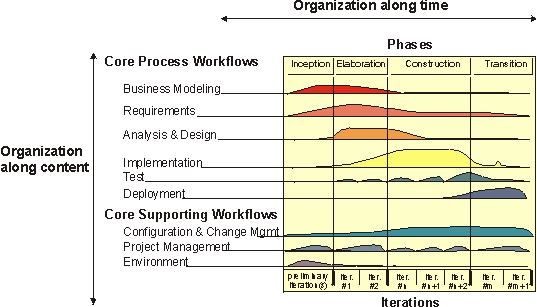
\includegraphics[width=12cm]{images/rup.png}
	\caption{Vista general de RUP}
	\label{fig:RUP}
\end{figure}

Las fases seguidas fueron:

\begin{enumerate}
  \item Inicio: se hizo un plan de fases, identificando los principales 
	casos de uso y riesgos.
  \item Elaboración: se hizo un plan de proyecto, completándose los casos 
	de uso para eliminar los riesgos.
  \item Construcción: se concentró en la elaboración de un producto totalmente 
	operativo y eficiente, así como en un pequeño manual de usuario.
  \item Transición: se publicaron varias versiones funcionales.
\end{enumerate}

Para cada fase RUP define nueve actividades a realizar:

\begin{enumerate}
 \item Modelado del negocio
 \item Análisis de requisitos
 \item Análisis y diseño
 \item Implementación
 \item Test
 \item Distribución
 \item Gestión de configuración y cambios
 \item Gestión del proyecto
 \item Gestión del entorno
\end{enumerate}

Además de un flujo de trabajo entre ellas es como se puede ver en la 
figura~\ref{fig:RUPWorkflow}\footnote{Imagen extraída del artículo
\url{http://www.javahispano.org/articles.article.action?id=76}}:

\begin{figure}[ht]
	\centering
	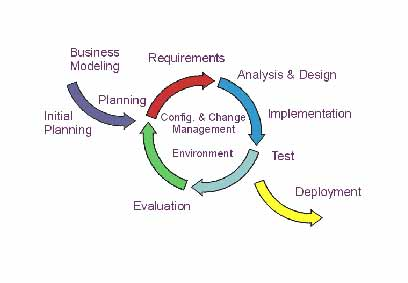
\includegraphics[width=9cm]{images/workflow-rup.png}
	\caption{Flujos de trabajo de RUP}
	\label{fig:RUPWorkflow}
\end{figure}

En RUP se utiliza UML\footnote{\url{http://www.omg.org/uml/}} como herramienta principal
para la documentación de toda la arquitectura del sistema. La bibliografía es amplia,
disponiendo de veteranos títulos como 
\emph{The Unified Modeling Language Reference Manual}\cite{UMLReference} o 
\emph{UML Distilled}\cite{UMLDistilled} como guías de referencia, siendo imprescindible
tener siempre a mano el \emph{UML 2.0 Pocket Reference}\cite{UMLPocket} para resolver
rápidamente esas consultas puntuales de la especificación.

RUP puede englobarse dentro de lo que algunos llaman \emph{procesos pesados},
estando quizás muy orientado para proyecto de algo más de envergadura que SWAML.
Aunque algunos autores\cite{Larman2004} ya incluyen RUP dentro de los llamados 
\emph{procesos ágiles}. Aún así, debido a las características del proyecto, 
(tamaño y personas involucradas) ha sido necesario hacer una pequeña adaptación 
de RUP utilizando sólo los documentos y procesos de diseños necesarios.

Este método es de sobra conocido y esta perfectamente documentado (en libros como
\emph{The Rational Unified Process}\cite{RUPIntro} y
\emph{The Rational Unified Process Made Easy}\cite{RUPEasy}) como para
extenderse más reescribiendo dicha documentación.
